% =============================================================================
% Supplementary material for
%   "A Blueprint for Cross-Modal Coordination at the Far Edge"
%
% Contains the artifacts that appeared in the submitted draft but were cut from
% the camera-ready for space. Referenced by the project-page footnote in §IV-A.
%
% Build:  tectonic -X compile supplement.tex     (or pdflatex twice)
% Shares figures/ with the main paper -- no files are duplicated.
% =============================================================================
\documentclass[conference]{IEEEtran}
\IEEEoverridecommandlockouts
\usepackage{cite}
\usepackage{amsmath,amssymb,amsfonts}
\usepackage{graphicx}
\usepackage{textcomp}
\usepackage{xcolor}
\usepackage{booktabs}
\usepackage{multirow}
\usepackage{tabularx}
\usepackage{subcaption}
\usepackage{enumitem}
\usepackage{url}

\usepackage{pifont}
\newcommand{\cmark}{\ding{51}}
\newcommand{\xmark}{\ding{55}}

% The shared fragments are written for the main paper and reference its
% sections. Resolve those to the printed section numbers of the paper rather
% than to anything in this document.
\newlabel{sec:fidelity}{{VI-A}{--}}
\newlabel{sec:6_synthesis-results}{{VI}{--}}
\newlabel{sec:case-study-results}{{VI-B}{--}}
\newlabel{sec:char-topology}{{V-D}{--}}
\newlabel{sec:limitations}{{VII-B}{--}}

\renewcommand{\thetable}{S\arabic{table}}
\renewcommand{\thefigure}{S\arabic{figure}}

\title{\Large \bf Supplementary Material for\\
``A Blueprint for Cross-Modal Coordination at the Far Edge''}

\author{\IEEEauthorblockN{Jenna Kline\textsuperscript{1,2}, Anirudh Potlapally\textsuperscript{1},
Yuanyang Cheng\textsuperscript{1}, Tanya Berger-Wolf\textsuperscript{1},\\
Hari Subramoni\textsuperscript{1}, and Christopher Stewart\textsuperscript{1}}
\IEEEauthorblockA{\textsuperscript{1}\textit{Dept. of Computer Science and Engineering, The Ohio State University}, Columbus, OH, USA \\
\textsuperscript{2}\textit{Dept. of Civil and Environmental Engineering, Massachusetts Institute of Technology}, Cambridge, MA, USA \\
Contact: kline.377@osu.edu}}

\begin{document}
\maketitle

\section{Scope}

This document collects the tables and figures that appeared in the submitted
version of the paper and were removed from the camera-ready for space. Nothing
here is new: every artifact is referenced from the main text, and the numbers
reproduce those reported in the paper. Section numbers cited below
(e.g.\ \S\ref{sec:fidelity}) refer to the main paper, not to this document.

The material is organized in the order it is used by the paper:

\begin{enumerate}[leftmargin=*,noitemsep]
  \item \textbf{Notation} (Table~\ref{tab:notation}) --- symbols used throughout
        the method (\S III).
  \item \textbf{Fidelity scorecard} (Table~\ref{tab:fidelity_scorecard}) ---
        summary of the three synthesis consistency checks (\S\ref{sec:fidelity}).
  \item \textbf{Operational fidelity detail}
        (Table~\ref{tab:operational_fidelity}) --- per-policy recorded vs.\
        synthesized comparison underlying \S VI-A.2.
  \item \textbf{Per-policy coverage--energy tradeoff}
        (Fig.~\ref{fig:pareto-policies}) --- the operating points the four
        inference policies admit (\S IV-C).
  \item \textbf{Variance envelope} (Fig.~\ref{fig:variance-envelope}) --- the
        nine modality $\times$ statistic cells behind the variance bound
        (\S VI-A.1).
  \item \textbf{Case-study takeaways} (Table~\ref{tab:case-takeaways}) ---
        configurations, verdicts, and provisioning takeaways for CS1--CS4
        (\S\ref{sec:case-study-results}).
  \item \textbf{Intensity sweep} (Fig.~\ref{fig:intensity-sweep}) --- synthesis
        under intensity scaling against natural per-site bounds (\S V-D.2).
\end{enumerate}

\noindent Analysis code and the derived per-modality event tables from which
these artifacts are generated are in the project repository.

\section{Notation}
\begin{table*}[b]
\centering
\footnotesize
\begin{tabular}{@{}ll@{}}
\toprule
\textbf{Symbol} & \textbf{Meaning} \\
\midrule
\multicolumn{2}{l}{\textit{Modalities and traces}} \\
$M$ & Set of recorded modalities \\
$T_m$ & Normalized per-modality trace, modality $m \in M$ \\
$\tau_m$ & Observation horizon of trace $T_m$ \\
\midrule
\multicolumn{2}{l}{\textit{Arrival behavior}} \\
$\{t_i\}$ & Change points partitioning $\tau_m$ \\
$R_{m,i}$ & Arrival rate of modality $m$ in segment $i$ \\
$\rho_m$ & Arrival process $\{(t_i, R_{m,i})\}_i$ for modality $m$ \\
$\mathrm{CV}_m$ & Coefficient of variation of $m$'s inter-arrival times \\
$B_m$ & Burstiness, $(\mathrm{CV}_m{-}1)/(\mathrm{CV}_m{+}1) \in [-1, 1]$ \\
\midrule
\multicolumn{2}{l}{\textit{Cross-modal and post-filter}} \\
$C_{m,m'}$ & Cross-modal co-occurrence (Jaccard) $\in [0, 1]$ \\
$\phi_m^{\mathrm{raw}}$ & Raw arrival rate of modality $m$ \\
$\phi_m^{\mathrm{det}}$ & Post-detection rate of modality $m$ \\
$\phi_m^{\mathrm{thr}}$ & Post-threshold rate of modality $m$ \\
$\phi_m$ & Throughput tuple $(\phi_m^{\mathrm{raw}}, \phi_m^{\mathrm{det}}, \phi_m^{\mathrm{thr}})$ \\
\midrule
\multicolumn{2}{l}{\textit{Workload model and synthesis}} \\
$\mathcal{W}$ & Workload model $\{\rho_m, B_m, C_{m,m'}, \phi_m\}_{m \in M}$ \\
$c$ & Configuration  \\
$c_{\mathrm{id}}$ & Identity recipe (baseline from real traces) \\
$s$ & Random seed \\
$T^*$ & Synthetic multimodal trace, $T^* = \mathrm{synth}(\mathcal{W}, c, s)$ \\
\midrule
\multicolumn{2}{l}{\textit{Fidelity statistics}} \\
$\mathrm{KS}_{\mathrm{diurnal}}$ & KS distance between hour-of-day arrival distributions \\
$\mathrm{spread}_s[\cdot]$ & Bootstrap 95\% interval across seeds \\
$\mathrm{spread}_{\mathrm{site}}[\cdot]$ & Bootstrap 95\% interval across recorded sites \\
\bottomrule
\end{tabular}
\caption{Framework Notation.}
\label{tab:notation}
\end{table*}
\clearpage

\section{Synthesis Fidelity}

Table~\ref{tab:fidelity_scorecard} summarizes the three consistency checks
reported in \S\ref{sec:fidelity}. These establish that synthesis is
self-consistent with the recorded traces; they are not a validation against a
deployed cross-modal system.

% Auto-generated by make_tab_fidelity_scorecard.py — do not edit by hand.
\begin{table}[t]
\centering\small
\begin{tabular}{@{}p{1.7cm} p{2.6cm} p{3.4cm}@{}}
\toprule
\textbf{Criterion} & \textbf{What it licenses} & \textbf{Result} \\
\midrule
Identity test & Re-emission of recorded distribution & \textbf{PASS} ($\Delta B_m \leq 0.10$ all modalities; max $= 0.092$, bioacoustic) \\
\addlinespace[2pt]
Variance bound & Distributional plausibility for synthesis recipes & \textbf{PASS} ($n_{\mathrm{pass}} = 9/9$; $W_{m,\theta} \in [0.002, 0.48]$) \\
\addlinespace[2pt]
Operational fidelity & Provisioning policy comparison & \textbf{PASS} (laptop tier; Kendall $\tau = 1.00$ on policy SLO ranking) \\
\addlinespace[2pt]
Generalization (derived) & What-if planning beyond recorded conditions & \textbf{PASS} (qualitative direction recovery; L2 sweep $n = 12/18$ cells in envelope) \\
\bottomrule
\end{tabular}
\caption{Synthesis fidelity scorecard. All three fidelity criteria pass on the
recorded traces; the derived generalization test recovers prior work's
directional shifts qualitatively. The bioacoustic identity deviation
($\Delta B = 0.092$) reflects two recording-schedule
regimes (hourly-clocked and chorus-only ARUs) being mixed in the modality-level
synthesis bootstrap; see \S\ref{sec:discussion} footnote.}
\label{tab:fidelity_scorecard}
\end{table}


Table~\ref{tab:operational_fidelity} gives the per-policy detail behind the
operational-fidelity check. Per-policy $p_{95}$ latency and SLO compliance match
between recorded and synthesized traces; total energy scales with event count
while per-event energy is invariant within a policy.

\begin{table*}[b]
\centering
\begin{tabular}{@{}l rrr rrr@{}}
\toprule
& \multicolumn{3}{c}{\textbf{Recorded}} & \multicolumn{3}{c}{\textbf{Synthesized}} \\
\cmidrule(lr){2-4} \cmidrule(lr){5-7}
\textbf{Policy} & $p_{95}$ (ms) & SLO (\%) & Energy (kJ) & $p_{95}$ (ms) & SLO (\%) & Energy (kJ) \\
\midrule
process-all & $100$ & $100$ & $95.4$ & $100$ & $100$ & $453.7$ \\
event-triggered & $100$ & $100$ & $9.9$ & $100$ & $100$ & $38.0$ \\
adaptive & $200$ & $100$ & $11.9$ & $200$ & $100$ & $12.0$ \\
control-theoretic & $200$ & $100$ & $9.9$ & $200$ & $100$ & $38.0$ \\
\bottomrule
\end{tabular}
\caption{Operational fidelity on the laptop tier: recorded strict camera trace
($n = 39\,742$ events) vs.\ identity-synthesized camera-only trace
($n \approx 189\,000$ events, mean over 3 seeds). Per-policy
$p_{95}$ latency and SLO compliance match exactly between recorded and
synthesized; total energy scales with event count and per-event energy is
exactly invariant ($2.40$\,J/event in all eight cells). Policy ranking by
$p_{95}$ latency is preserved exactly (Kendall $\tau = 1.0$).}
\label{tab:operational_fidelity}
\end{table*}

\begin{figure*}[htp]
    \centering
    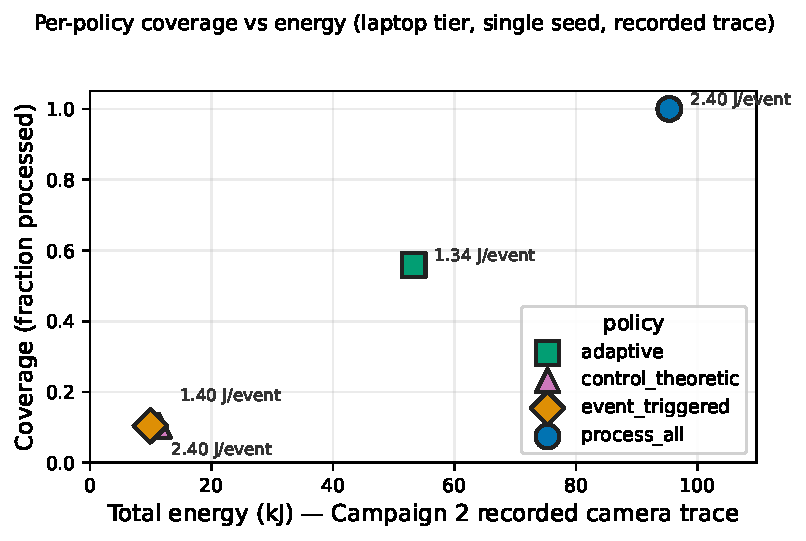
\includegraphics[width=0.8\linewidth]{figures/fig_08_pareto_policies.pdf}
    \caption{Per-policy coverage--energy tradeoff on the recorded camera trace at the field-laptop tier.}
  \label{fig:pareto-policies}
\end{figure*}

\begin{figure*}
    \centering
    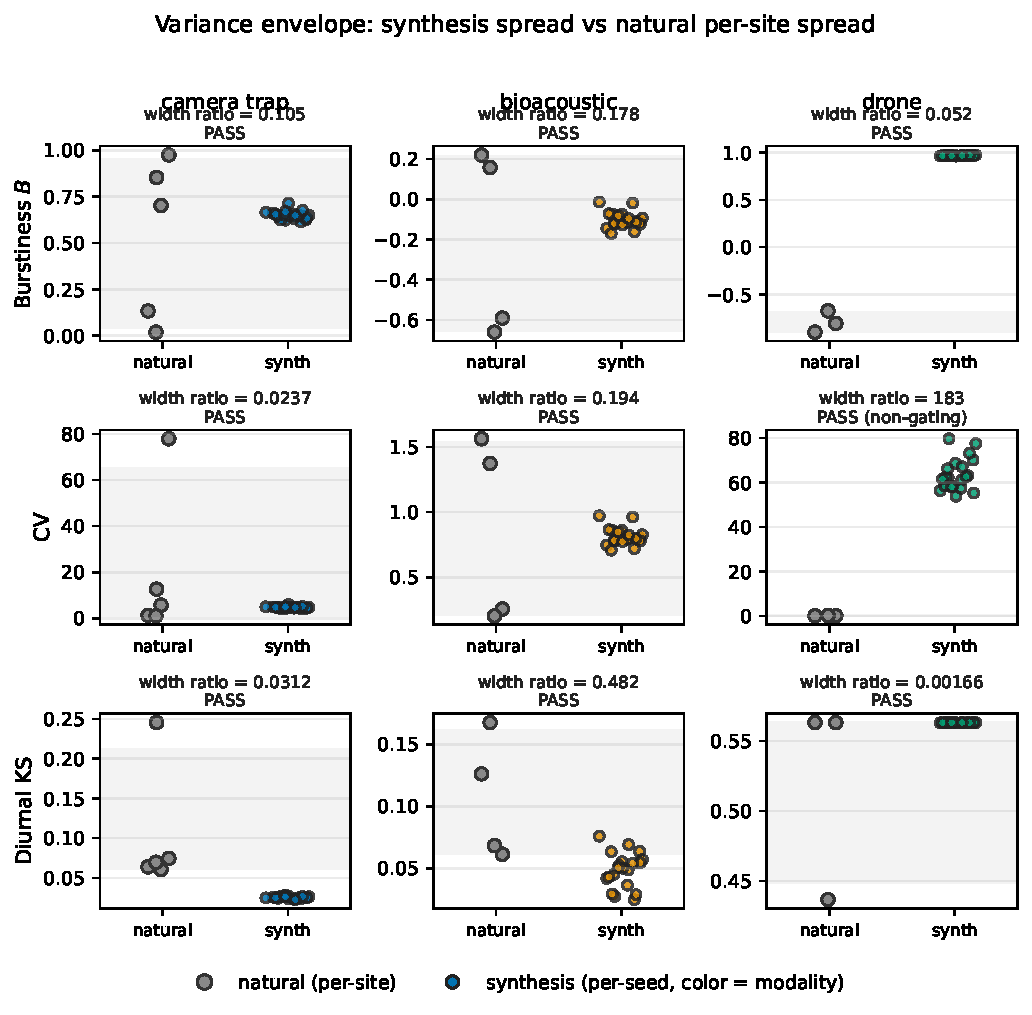
\includegraphics[width=1\linewidth]{figures/fig_app_03_variance_envelope.pdf}
    \caption{Variance envelope across modality $\times$ statistic bins. All 9 cells satisfy $\mathrm{spread}_s[\theta(T^*)] \leq \mathrm{spread}_\mathrm{site}[\theta(T_m)]$.}
  \label{fig:variance-envelope}
\end{figure*}
\clearpage

\section{Case-Study Detail}

% =============================================================================
% Table: case-study takeaways
% =============================================================================
% One row per case, three substantive columns:
%   (1) Recipe summary
%   (2) Feasibility verdict (compact)
%   (3) Provisioning takeaway (single sentence)
%
% Sourced from §VI.B prose. Designed to be the "table you read instead of
% the section if you only have 30 seconds."
%
% Layout: table* (two-column-spanning) since the provisioning takeaways need
% horizontal space to read. If single-column is required, drop to \small and
% truncate the takeaways or use \makecell for line breaks within cells.
% =============================================================================

\begin{table*}[t]
  \centering
  \small
  \begin{tabular}{p{0.04\textwidth} p{0.20\textwidth} p{0.30\textwidth} p{0.36\textwidth}}
    \toprule
    \textbf{Case} & \textbf{Configuration} & \textbf{Feasibility verdict} & \textbf{Provisioning takeaway} \\
    \midrule
    CS1 & Bioacoustic $\rightarrow$ camera trap; conditional scaling (assumed $2\times$ for $60$\,s post-trigger); 2\,s SLO. & RTX, Jetson feasible. Laptop infeasible (CPU latency). Pi5+TPU structurally unsupported (no Edge TPU path for MegaDetector). Pi4 infeasible (CPU latency). & Jetson is the minimum tier under a 2\,s SLO regardless of bioacoustic schedule. Schedule choice (hourly vs.\ chorus) is a workload-design lever that shapes response-tier sizing. \\
    \addlinespace
    CS2 & Camera trap $\rightarrow$ drone; interleave with response delay $\sim \mathcal{U}[0.1, 5.0]$\,s; 5\,s SLO. & RTX, Jetson, Pi5+TPU, Pi4 all feasible. Laptop infeasible; verdict confirmed empirically (\S\ref{sec:fidelity}, $+23.4\%$ measured-vs-predicted gap). & Pi-class hardware is predicted feasible at this SLO; drone-side inference is not the binding constraint. The field laptop is the limiting tier --- not a more capable alternative. \\
    \addlinespace
    CS3 & Focal CT $\rightarrow$ CT network; conditional scaling (assumed $1.5\times$ neighbor density for $10$\,s); 10\,s SLO. & RTX, Jetson, Pi5+TPU, Pi4 all feasible. Laptop infeasible (latency overrun + queue overflow). & Gateway-tier capacity must be sized against the two-site worst case, not an asymptotic full-network average --- camera-trap sites share diurnal structure. \\
    \addlinespace
    CS4 & Citsci $\rightarrow$ all; prior injection (assumed $1.25\times$ density boost during $60$\,s post-citsci windows); 60\,s SLO. & Feasible on all five tiers. Laptop reaches $43.6\%$ MegaDetector utilization under adaptive policy. & Citsci-as-prior does not stress edge-tier compute at the densities evaluated. Size the gateway-tier ingestion pipeline against the citsci arrival rate, scaled by the prior's spatial granularity. \\
    \bottomrule
  \end{tabular}
  \caption{Case-study takeaways. Configurations, feasibility verdicts, and provisioning takeaways for the four configurations.}
  \label{tab:case-takeaways}
\end{table*}


\begin{figure*}
    \centering
    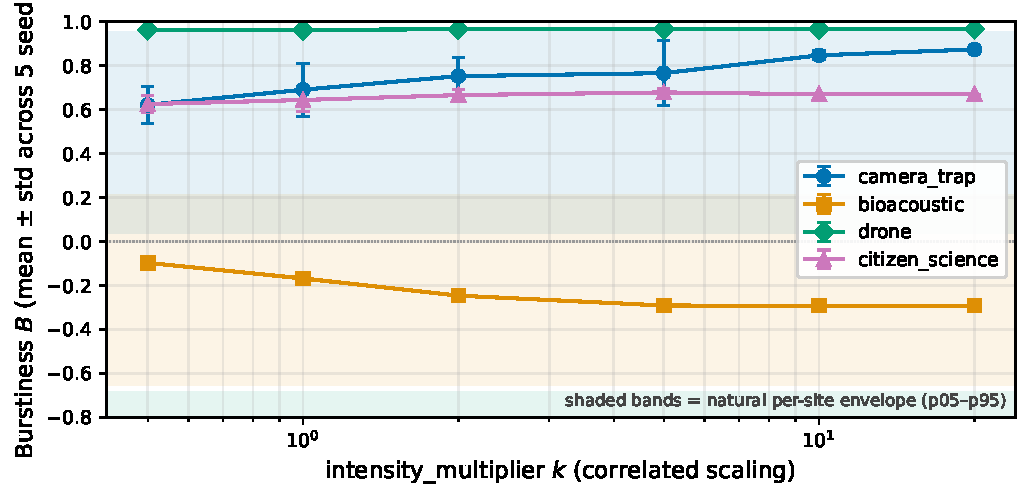
\includegraphics[width=1\linewidth]{figures/fig_app_04_intensity_sweep.pdf}
    \caption{Synthesis under intensity scaling $r_k$ for $k \in \{0.5, 1, 2, 5, 10, 20\}$, compared against natural per-site bounds (shaded).}
  \label{fig:intensity-sweep}
\end{figure*}

\end{document}
